% allgemeine Voreinstellungen
% ****************************************************************
\pagestyle{scrheadings}

% Layoutfestlegungen
% ****************************************************************
\definecolor{chapter}{rgb}{0,0.25,0.56}
\definecolor{section}{rgb}{0.27,0.33,0.90}
\definecolor{subsection}{rgb}{0.54,0.66,0.90}
\definecolor{subsubsection}{rgb}{0.14,0.17,0.95}
\definecolor{paragraph}{cmyk}{0.5,0,.1,.39}

\addtokomafont{chapter}{\color{chapter}}
\addtokomafont{section}{\color{section}}
\addtokomafont{subsection}{\color{subsection}}
\addtokomafont{subsubsection}{\color{subsubsection}}
\addtokomafont{paragraph}{\color{paragraph}}

\hypersetup{
    hidelinks
}

% Kopfzeile festlegen
% ****************************************************************
% Kopf, Innenseite
\ihead{\leftmark}

% Kopf, Mitte
\chead{}

% Kopf, Außenseite
\ohead{\Titel}

% Aufgabeneinstellungen
\DeclareExerciseEnvironmentTemplate{schule-leitprogramm}
{%
\tcolorbox[
	colback = grey9,
	colframe = grey9,
	sharp corners,
	coltitle = black,
	flushleft title,
	bottomtitle=0mm,
	boxsep=0.5mm,
	top=0.5mm,
	bottom=1mm,
    breakable,
	title = \uebungBild \GetExerciseName~\GetExerciseProperty{chapter}.\GetExerciseProperty{counter}%
        \hfill%
        \ifthenelse{\boolean{schule@hinweislink}}{%
            \GetExercisePropertyT{bearbeitungshinweis}{\hyperref[hinweis:\ExerciseID]{\colorbox{black!30}{\color{blue!90}H}}}%
        }{}%
        \ifthenelse{\boolean{schule@loesunglink}}{%
            \IfExistSolutionT{~\hyperref[loesung:\ExerciseID]{\colorbox{black!30}{\color{blue!90}L}}}%
        }{}%
	]%
	\label{aufgabe:\ExerciseID}
}
{\endtcolorbox}

\DeclareExerciseEnvironmentTemplate{schule-leitprogramm-loesung} {%
    \addpenalty{-3000}\smallskip\noindent\textbf{%
        % Falls Zusatzaufgabe:
        %   \llap{\GetExerciseProperty{symbol}}
        \ifthenelse{\equal{\ExerciseType}{zusatzaufgabe}}{\llap{\GetExerciseProperty{symbol}$\bigstar$}~}{\llap{\GetExerciseProperty{symbol}~}}%
        \XSIMmixedcase{\GetExerciseName}\nobreakspace
        \GetExerciseProperty{chapter}.\GetExerciseProperty{counter}\label{loesung:\ExerciseID}\hfill\hyperref[aufgabe:\ExerciseID]{\colorbox{black!30}{\color{blue!90}$\leftarrow$}}%
    }\par\smallskip
}
{\par}%

\xsimsetup{
	aufgabe/template=schule-leitprogramm,
	aufgabe/within=chapter,
    loesung/template=schule-leitprogramm-loesung,
    print-solutions/headings=false,
}

\definecolor{grey1}{rgb}{.1,.1,.1}
\definecolor{grey2}{rgb}{.2,.2,.2}
\definecolor{grey3}{rgb}{.3,.3,.3}
\definecolor{grey4}{rgb}{.4,.4,.4}
\definecolor{grey5}{rgb}{.5,.5,.5}
\definecolor{grey7}{rgb}{.7,.7,.7}
\definecolor{grey8}{rgb}{.8,.8,.8}
\definecolor{grey9}{rgb}{.9,.9,.9}

\newcommand{\uebungBild}{

\begin{tikzpicture}[y=0.80pt, x=0.8pt,yscale=-1, inner sep=0pt, outer
sep=0pt] \path[draw=grey5,fill=grey7,line join=miter,line
cap=butt,line width=0.209pt] (12.0208,0.5895) --
(1.3666,3.8375) -- (3.3843,20.6431) -- (20.4113,14.4179) --
cycle; \path[draw=grey1,fill=grey9,line join=round,line
cap=butt,line width=0.209pt] (7.1932,6.1991) --
(15.9622,12.7759) -- (16.8321,11.7667) -- (7.8544,5.3292) --
cycle; \path[draw=grey1,fill=grey3,line join=round,line
cap=butt,line width=0.209pt] (7.8544,5.3292) --
(5.9231,4.7550) -- (7.1932,6.1991) -- cycle;
\end{tikzpicture}
}

\newcommand{\hinweisBild}{
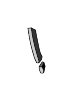
\begin{tikzpicture}[y=0.80pt, x=0.8pt,yscale=-1, inner sep=0pt, outer
sep=0pt] \path[draw=black,fill=grey2,line join=miter,line
cap=butt,miter limit=4.00,line width=0.160pt] (6.4521,1.4334)
-- (7.4295,0.4560) .. controls (7.9473,0.7196) and
(8.1724,0.8553) .. (9.3447,1.4053) .. controls (9.3447,1.4053)
and (9.4550,2.1225) .. (9.7278,3.7868) .. controls
(9.7547,3.9511) and (10.4938,7.4506) .. (10.4938,7.4506) ..
controls (10.4938,7.4506) and (11.0227,10.4067) ..
(11.5264,11.8139) .. controls (11.7222,12.3609) and
(12.1912,12.8073) .. (12.2925,13.3794) .. controls
(12.3294,13.5882) and (12.2747,13.8058) .. (12.2258,14.0122)
.. controls (12.1526,14.3214) and (12.0628,14.5394) ..
(11.8899,14.9041) .. controls (11.5477,15.6258) and
(10.6101,16.3538) .. (10.6271,16.2438);
\path[draw=black,fill=grey8,line join=round,line cap=butt,line
width=0.200pt] (5.8974,0.5893) -- (7.4295,0.4519) .. controls
(8.0049,6.9583) and (10.9185,15.1671) .. (10.8935,15.6401) ..
controls (10.8820,15.8585) and (10.8157,16.1331) ..
(10.6271,16.2438) .. controls (10.4156,16.3680) and
(10.0239,16.3854) .. (9.8943,16.1772) .. controls
(8.7782,14.3840) and (8.5425,12.9279) .. (8.0291,11.2477) ..
controls (7.4491,9.3496) and (7.0458,7.3997) ..
(6.6635,5.4522) .. controls (6.3474,3.8419) and
(5.8974,0.5893) .. (5.8974,0.5893) -- cycle;
\path[draw=black,fill=black,line join=round,line
cap=butt,miter limit=4.00,line width=0.160pt]
(13.0918,15.9107) -- (13.6664,17.7926) -- (13.0575,20.6334) --
(11.7179,19.3081) -- (13.0918,15.9107);
\path[draw=black,fill=grey4,line join=round,line
cap=butt,miter limit=4.00,line width=0.160pt]
(13.0918,15.9107) -- (12.1925,18.0424) -- (10.8935,18.0424) --
(12.3258,15.7775) -- cycle; \path[draw=black,fill=grey8,line
join=round,line cap=butt,miter limit=4.00,line width=0.160pt]
(10.8935,18.0424) .. controls (10.8935,18.0424) and
(11.1714,19.7148) .. (11.1600,19.6412) .. controls
(11.0947,19.2217) and (11.1324,20.0124) .. (11.7262,20.8070)
.. controls (11.9101,21.0529) and (12.7921,20.8070) ..
(12.9586,20.7403) .. controls (13.1251,20.6737) and
(12.9586,19.3414) .. (12.9586,19.3414) -- (12.1925,18.0424) --
cycle;
\end{tikzpicture}
}

\newmdenv[backgroundcolor=grey9,linewidth=0pt]{grey@Frame}

\makeatletter% siehe FAQ (aber wirklich nachsehen!)
\newcommand*{\headingpar}{\par\nobreak\@afterheading}
\makeatother% siehe FAQ

\newenvironment{greyFrame}[2]%
{\begin{grey@Frame}#1
 \raisebox{+0.9ex}{
  \begin{large}#2\end{large}
 }\vspace*{-0.2cm}\headingpar}%
{\end{grey@Frame}}

\newenvironment{hinweisBox}%
{\begin{greyFrame}{\hinweisBild{}}{Hinweis}}%
{\end{greyFrame}}%


%Monatsname für z.B. Titelblatt
\newcommand{\monatWort}[1]{%
    \IfInteger{#1}{%
        \ifcase #1
            Monat 0 \or Januar \or Februar \or März  \or April \or Mai \or Juni \or Juli %
            \or August \or September \or Oktober \or November \or Dezember \fi%
    }{Unbekannter Monat}%
}

%TextFeld in das Ergebnisse eingetragen werden können
\newcommand{\TextFeld}[1]{%
    \par\smallskip
    \begin{Form}
    \TextField[width=\linewidth,%
    height=#1,multiline=true,borderwidth=0]{}%
    \end{Form}
}%

% Ausgabe von Hinweisen
% modifiziert für das Leitprogramm
% ********************************************************************

% Vollständige Liste
\renewcommand{\bearbeitungshinweisliste}{
    \ForEachUsedExerciseByType{%
        \def\ExerciseType{##1}%
        \def\ExerciseID{##2}%
        \GetExercisePropertyT{bearbeitungshinweis}{%
            \addpenalty{-3000}\smallskip\noindent\textbf{%
                Hinweis zu \XSIMmixedcase{\GetExerciseName}~\GetExerciseProperty{chapter}.##3\label{hinweis:##2}\hfill\hyperref[aufgabe:\ExerciseID]{\colorbox{black!30}{\color{blue!90}$\leftarrow$}}%
            }\par\smallskip
            ####1 \par%
        }%
    }%
}
